\chapter{Descriptive overview of Edit Filters on the English Wikipedia}
\label{chap:overview-en-wiki}

The purpose of this chapter (syn?) is to explore the edit filters on the Englisch Wikipedia.
We want to gather a understanding of what types of tasks these filters take over,
and, as far as feasible, trace how these tasks have evolved over time.

%TODO describe what each section is about
The data upon which the analysis is based is described in section~\ref{sec:overview-data}
and the methods used–in chapter~\ref{chap:methods}.
We look into the manual classification of EN Wikipedia's edit filters I've undertaken in an attempt to understand what is it that they actually filter in section~\ref{sec:manual-classification}.
Section~\ref{sec:patterns} studies some general characteristics of the edit filters, whereas their activity is analysed in section~\ref{sec:filter-activity}.
And finally, some historical patterns are observed in section~\ref{sec:5-history}.

%TODO tell a story with the chapter: what do filters do? How have their tasks evolved over time (if feasible) --> maybe tell it along the peak: it is an extraordinary situation, where we can see it is exactly X and Y and Z what filters do


\section{Data}
\label{sec:overview-data}

A big part of the present analysis is based upon the \emph{abuse\_filter} table from \emph{enwiki\_p}(the database which stores data for the EN Wikipedia), or more specifically a snapshot thereof which was downloaded on January 6th, 2019 via quarry, a web-based service offered by Wikimedia for running SQL queries against their public databases~\footnote{\url{https://quarry.wmflabs.org/}}.
The complete dataset can be found in the repository for the present paper~\cite{github}. % TODO add a more specific link
This table, along with \emph{abuse\_filter\_actions}, \emph{abuse\_filter\_log}, and \emph{abuse\_filter\_history}, are created and used by the AbuseFilter MediaWiki extension~(\cite{gerrit-abusefilter-tables}), as discussed in section~\ref{sec:mediawiki-ext}.

Selected queries have been run via quarry against the \emph{abuse\_filter\_log} table as well.
These are the foundation for the filters activity analysis undertaken in section~\ref{sec:filter-activity}.
Unfortunately, the \emph{abuse\_filter\_history} table which will be necessary for a complete historical analysis of the edit filters is currently not exposed to the public due to security/privacy concerns~\cite{phabricator}.
%TODO footnote about the submitted patch
Hence, in section~\ref{sec:5-history} the present work only touches upon historical trends in a qualitative fashion. %TODO how are these determined: API to abuse_filter_history; general stats from abuse_filter
or qualitatively shows patterns.
A comprehensive historical analysis is therefore one of the directions for future research discussed in section~\ref{sec:further-studies}.

A concise description of the tables has been offered in section~\ref{sec:mediawiki-ext} which discusses the AbuseFilter MediaWiki extension in more detail.
For further reference, the schemas of all four tables can be viewed in figures~\ref{fig:app-db-schemas-af},~\ref{fig:app-db-schemas-afl},~\ref{fig:app-db-schemas-afh} and~\ref{fig:app-db-schemas-afa} in the appendix.

%TODO think about the name of the section
\section{Types of edit filters: Manual Classification}
\label{sec:manual-classification}

In order to get a better understanding of what exactly it is that edit filters are filtering, I applied a grounded theory inspired emergent coding(see chapter~\ref{chap:methods}) to all filters, scrutinising their patterns, comments and actions.
Three big clusters of codes were identified, namely ``vandalism'', ``good faith'', and ``maintenance'', as well as the auxiliary cluster ``unknown''.
These are discussed in more detail later in this section, but first the coding itself is presented.

\subsection{Coding process and challenges}

As already mentioned, I started coding strongly influenced by the coding methodologies applied by grounded theory scholars (see section~\ref{sec:gt}) and let the labels emerge during the process.
I looked through the data paying special attention to the name of the filters (``af\_public\_comments'' field of the \emph{abuse\_filter} table), the comments (``af\_comments''), the regular expression pattern constituting the filter (``af\_pattern''), and the designated filter actions (``af\_actions'').

The assigned codes emerged from the data: some of them being literal quotes of terms used in the decription or comments of a filter, while others summarised the perceived filter functionality.
In addition to that, for vandalism related labels, I used some of the vandalism types identified by the community in~\cite{Wikipedia:VandalismTypes}.
However, this typology was regarded more as an inspiration instead of being adopted 1:1 since some of the types were quite general whereas more specific categories seemed to render more insights.
For instance, I haven't applied the ``addition of text'' category since it seemed more useful to have more specific labels such as ``hoaxing'' or ``silly\_vandalism'' (check the code book in the appendix~\ref{app:code_book} for definitions).
Moreover, I found some of the proposed types redundant.
For example, ``sneaky vandalism'' seems to overlap partially with ``hoaxing'' and partially with ``sockpuppetry'', ``link vandalism'' mostly overlaps with ``spam'' or ``self promotion'' (although not always), and for some reason, ``personal attacks'' are listed twice.

I have labeled the dataset twice.
The motivation therefor was to return to it once I've gained better insight into the data and use this newly gained knowledge to re-evaluate ambiguous cases, i.e. re-label some data with codes that emerged later in the process.
This mode of labeling is congruous with the simultaneous coding and data analysis suggested by grounded theorists (compare section~\ref{sec:gt}).

%1st labeling
Following challenges were encountered during the first round of labeling:
There were some ambiguous cases which I either tagged with the code I deemed most appropriate and a question mark, or assigned all possible labels (or both).
There were also cases for which I could not gather any insight relying on the name, comments and pattern, since the filters were hidden from public view and the name was not descriptive enough.
However, upon some further reflection, I think it is safe to assume that all hidden filters target a form of (more or less grave) vandalism, since the guidelines suggest that filters should not be hidden in the first place unless dealing with cases of persistent and specific vandalism where it could be expected that the vandalising editors will actively look for the filter pattern in their attempts to circumvent the filter\cite{Wikipedia:EditFilter}.
Therefore, during the second round of labeling I tagged all hidden filters for which there weren't any more specific clues (for example in the name of the filter) as ``hidden\_vandalism''.
And then again, there were also cases, not necessarily hidden, where I could not determine any suitable label, since I didn't understand the regex pattern, and/or none of the existing categories seemed to fit, and/or I couldn't think of an insightful new category to assign.
During the first labeling, these were labeled ``unknown'', ``unclear'' or ``not sure''.
For the second round, I have unified all of them under ``unclear''.

For a number of filters, it was particularly difficult to determine whether they were targeting vandalism or good faith edits.
The only thing that would have distinguished between the two would have been the contributing editor's motivation, which we had no way of knowing.
During the first labeling session, I tended to label such filters with ``vandalism?, good\_faith?''.
For the second labeling, I stuck to the ``assume good faith'' guideline~\cite{Wikipedia:GoodFaith} myself
and only labeled as vandalism cases where good faith was definitely out of the question.
One feature which guided me here was the filter action which represents the judgement of the edit filter manager(s).
Since communication is crucial when assuming good faith, all ambiguous cases which have a less ``grave'' filter action such as ``tag'' or ``warn'' (which seeks to give feedback and thereby effect/influence a constructive contribution) have received a ``good\_faith'' label.
On the other hand, filters set to ``disallow'' were tagged as ``vandalism'' or a particular type thereof, since the filter action is a clear sign that at least the edit filter managers have decided that seeking a dialog with the offending editor is no longer an option. %TODO check whether that's really the case

For the second round of labeling, I tagged the whole dataset again using the compiled code book (see \ref{app:code_book}) and assigned to every filter exactly one label–the one deemed most appropriate (although oftentimes alternative possibilites were listed as notes), without looking at the labels I assigned the first time around.
I intended to compare the labels from both coding sessions and focus on more ambiguous cases, re-evaluting them using all available information (patterns, public comments, labels from both sessions, as well as any notes I made along the line).
Unfortunately, there was no time, so the analysis of the present section is based upon the second round of labeling.
Comparing codes from both labeling sessions and refining the coding is one of the possibilities for future research. %TODO (re-formulate!)

%TODO disclose links to 1st and 2nd labelling
First round of labeling is available under \url{https://github.com/lusy/wikifilters/blob/master/filter-lists/20190106115600_filters-sorted-by-hits-manual-tags.csv}.

\begin{comment}
% Kept as a possible alternative wording for private vs public and labeling decisions in ambiguous cases
It was not always a straightforward decision to determine what type of edits a certain filter is targeting.
This was of course particularly challenging for private filters where only the public comment (name) of the filter was there to guide the coding.
On the other hand, guidelines state up-front that filters should be hidden only in cases of particularly persistent vandalism, in so far it is probably safe to establish that all hidden filters target some type of vandalism.
However, the classification was difficult for public filters as well, since oftentimes what makes the difference between a good-faith and a vandalism edit is not the content of the edit but the intention of the editor.
While there are cases of juvenile vandalism (putting random swear words in articles) or characters repetiton vandalism which are pretty obvious, that is not the case for sections or articles blanking for example.
For these, from the edit alone there is no way of knowing whether the deletion was malicious or the editor conducting it just wasn't familiar with say the correct procedure for moving an article.
\end{comment}

%TODO axial coding: sounds a bit lame still?
At the end, an axial coding phase took place in which the identified codes were sorted and unified into broader categories which seemed to relate the single labels to each other.
As signaled at the beginning of the section, following four categories were identified (syn): ``vandalism'', ``good faith'', ``maintenance'', and ``unknown''.
The subsections that follow discuss the salient properties of each of them.

\subsection{Vandalism}

The vast majority of edit filters on EN Wikipedia could be said to target (different forms of) vandalism, i.e. maliciously intended disruptive editing.
Some examples thereof are filters for juvenile types of vandalism (inserting swear or obscene words or nonsence sequences of characters into articles), for hoaxing (inserting obvious or less obvious false information in articles), for template vandalism (modifying a template in a disruptive way which is quite severe, since templates are displayed on various pages), or for spam (inserting links to promotional content, often not related to the content being edited). %TODO stick to one terminology; no "juvenile" vandalism otherwise
All codes belonging to the vandalism category together with definition and examples can be consulted in the code book attached in the appendix~\ref{app:code_book}.

Some vandalism types seem to be more severe than others (e.g. sock puppetry or persistent long term vandals).
It is mostly in these cases that the implemented filters are hidden.
Labels refering to such types of vandalism form their own subcategory: ``hardcore vandalism''. %TODO think about naming
It should be mentioned at this point that I also classified ``harassment'' and ``personal attacks'' as ``hardcore vandalism'', since these types of edits are highly harmful and often dealt with by hidden filters, although according to~\cite{Wikipedia:Vandalism} both behaviours are disruptive editing rather than vandalism and should generally be handled differently.

\subsection{Good Faith}

The second biggest category identified (syn!) were filters targeting (mostly) disruptive but not necessarily made with bad intentions edits.
The adopted name ``good faith'' is a term used/utilised by the Wikipedia community itself, most prominently in the guideline ``assume good faith''~\cite{Wikipedia:GoodFaith}.
Filters from this category mostly target unconstructive edits done by new editors, not familiar with syntax, norms, or guidelines which results in broken syntax, disregard of established processes (e.g. deleting something without running it through an Articles for Deletion process, etc.) or norms (e.g. copyright violations),  or unencyclopedic edits (e.g. without sources/with improper sources; badly styled; or with a skewed point of view).

The focus of these filters lies in the communication with the disrupting editors:
a lot of the filters issue warnings intending to guide the editors towards ways of modifying their contribution to become a constructive one.

Codes from this category often take into consideration the area the editor was intending to contribute to or respectively that they (presumably) unintentionally disrupted.


\subsection{Maintenance}

Some of the encountered edit filters on the EN Wikipedia were targeting neither vandalism nor good faith edits.
Rather, they had their focus on (semi-)automated routine (clean up) tasks.
These form the ``maintenance'' category.
Some of the filters target for instance bugs such as broken syntax caused by a faulty browser extension.
Or there are such which simply track particular behaviours (such as mobile edits or edits made by unflagged bots) for various purposes.

The ``maintenance'' category differs conceptually from the ``vandalism'' and ``good faith'' ones in so far that the logic behind it isn't editors' intention, but rather ``side''-occurances that mostly went wrong.

I've also grouped here various test filters (used by individual editors or share used by all editors).

\subsection{Unknown}

This is an auxiliary category comprising the ``unknown'' and ``misc'' codes %TODO allign with code book, right now there are 3 tags in the unknown cluster
used to code all filters where the functionality stayed completely opaque for the observer or although it was comprehensible what the filter was doing still no better fitting label emerged.

%************************************************************

%\section{Descriptive statistics/Patterns/General traits of the filters}
\section{Filter characteristics}
\label{sec:patterns}

In this section, we explore some general traits/patterns of/trends in the edit filters on Engish Wikipedia, or respectively the data from the \emph{abuse\_filter} table.
The scripts that generate the statistics (syn?) discussed here, can be found in the jupyter notebook in the project's repository. %TODO add link after repository has been cleaned up


\subsection{General traits}

As of January 6th, 2019 there are $954$ filters in the \emph{abuse\_filter} table.
It should be noted, that if a filter gets deleted, merely a flag is set to indicate so, but no entries are removed from the database.
So, the above mentioned $954$ filters are all filters ever made up to this date.
This doesn't mean that it never changed what the single filters are doing, since edit filter managers can freely modify filter patterns, so at some point the filter could be doing one thing and in the next moment it can be filtering a completely different phenomenon.
There are cases of filters being ``repurposed'' or modified to filter for example a more general occurance/phenomenon.
This doesn't happen very often though.
Mostly, if a filter is not useful anymore it is just disabled and eventually deleted and new filters are implemented for current problems.

$361$ of all filters are public, the remaining $593$–hidden.
$110$ of the public ones are active, $35$ are disabled, but not marked as deleted, and $216$ are flagged as deleted.
Out of the $593$ hidden filters $91$ are active, $118$ are disabled (not deleted), and $384$ are deleted.
The relative proportion of these groups to each other can be viewed on figure~\ref{fig:general-stats}.

\begin{figure}
\centering
  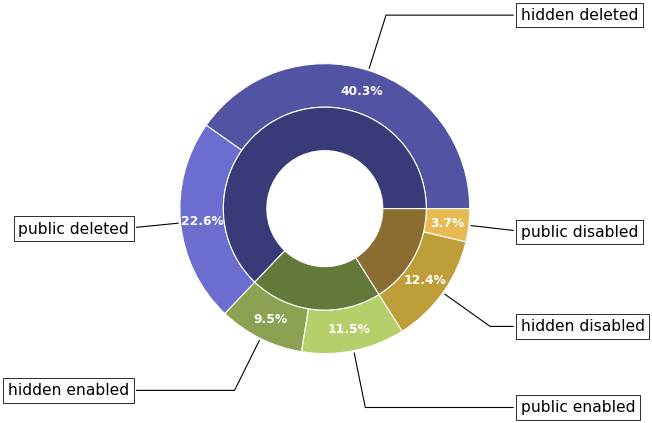
\includegraphics[width=0.9\columnwidth]{pics/general-stats-donut.png}
  \caption{There are 954 edit filters on EN Wikipedia}~\label{fig:general-stats}
\end{figure}

\subsection{Public and Hidden Filters}
\label{sec:public-hidden}

As signaled in section~\ref{section:4-history}, historically it was planed to make all edit filters hidden from the general public.
The community discussions rebutted that so a guideline was drafted calling for hiding filters
``only where necessary, such as in long-term abuse cases where the targeted user(s) could review a public filter and use that knowledge to circumvent it.''~\cite{Wikipedia:EditFilter}.
This is however not always complied with and edit filter managers do end up hiding filters that target general vandalism despite consensus that these should be public~\cite{Wikipedia:PrivacyGeneralVandalism}.
Such cases are usually made public eventually (examples hereof are filters 225 ``Vandalism in all caps'', 260 ``Common vandal phrases'', or 12 ``Replacing a page with obscenities'').
Also, oftentimes when a hidden filter is marked as ``deleted'', it is made public. %TODO examples?
%TODO this seems out of place
Further, caution in filter naming is suggested for hidden filters and editors are encouraged to give such filters just simple description of the overall disruptive behaviour rather than naming a specific user that is causing the disruptions.
(The latter is not always complied with, there are indeed filters named after the accounts causing a disruption.)

Still, it draws attention that currently nearly $2/3$ of all edit filters are not viewable by the general public (compare figure~\ref{fig:general-stats}).
Unfortunately, without the full \emph{abuse\_filter\_history} table we cannot know how this ration has developed historically.
However, the numbers fit the assertion of the extension's core developer according to whom edit filters target particularly determined vandals.

On the other hand, if we look at the enabled filters only, there are actually more or less the same number of public enabled and hidden enabled filters ($110$ vs $91$).
This leads to the hypothesis that it is rather that hidden filters have higher fluctuation rates, i.e. that they target specific phenomena that are over after a particular period of time after which the filters get disabled and eventually–deleted.
This makes sense when we compare it to the hidden vs public filter policy: hidden filters for particular cases and very determined vandals, public filters for general patterns which reflect more timeless patterns.


\subsection{Filter actions}

Another interesting parameter we could observe are the currently configured filter actions for each filter.
Figure~\ref{fig:all-active-filters-actions} depicts the actions configured for all enabled filters.
And figures~\ref{fig:active-public-actions} and~\ref{fig:active-hidden-actions} show the actions of all enabled public and hidden filters respectively.
It is noticeable that the most common action for the enabled hidden filters is ``disallow'' whereas most enabled public filters are set to ``tag'' or ``tag,warn''.
This is congruent with the community's claim that hidden filters target particularly perstistent vandalism, which is best outright disallowed.
A lot of public filters on the other hand still assume good faith from the editors and try to dissuade them from engaging in disruptive behaviour by using warnings or just tag conspicious behaviour for further investigation.

\begin{figure}
\centering
  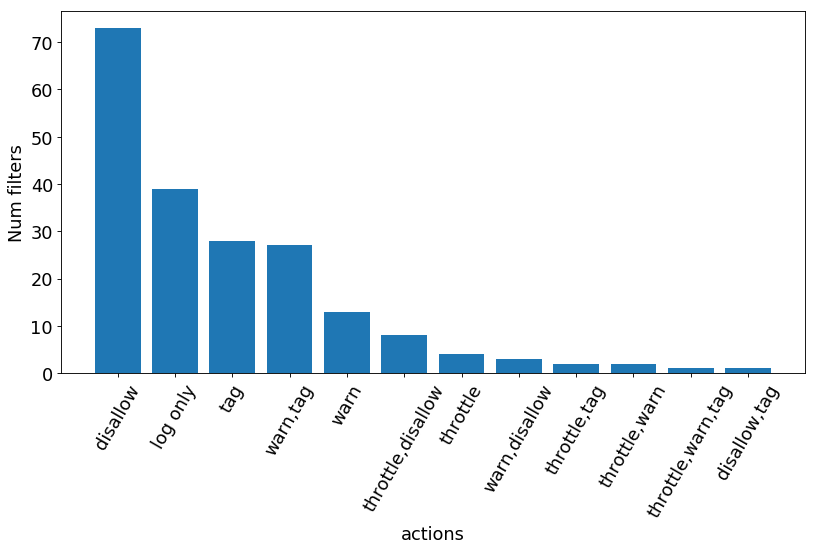
\includegraphics[width=0.9\columnwidth]{pics/all-active-filters-actions.png}
  \caption{EN Wikipedia edit filters: Filters actions for all filters}~\label{fig:all-active-filters-actions}
\end{figure}

\begin{figure}
\centering
  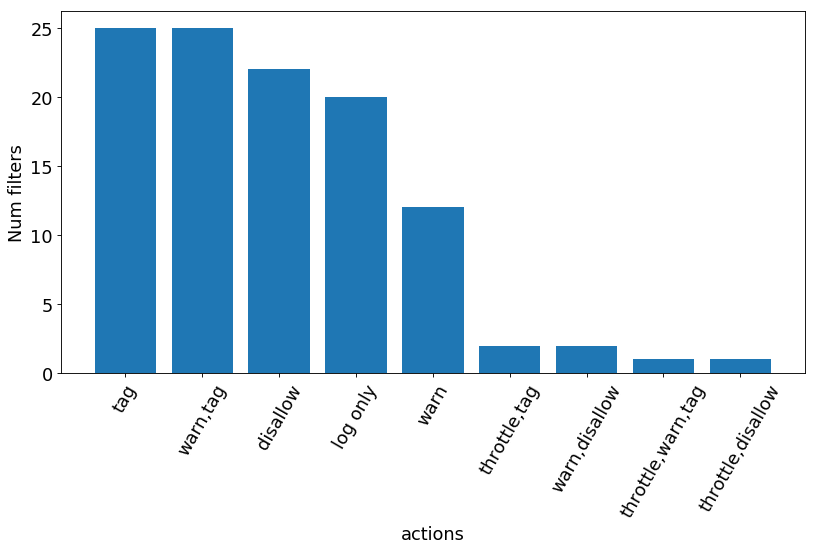
\includegraphics[width=0.9\columnwidth]{pics/active-public-actions-big.png}
  \caption{EN Wikipedia edit filters: Filters actions for enabled public filters}~\label{fig:active-public-actions}
\end{figure}

\begin{figure}
\centering
  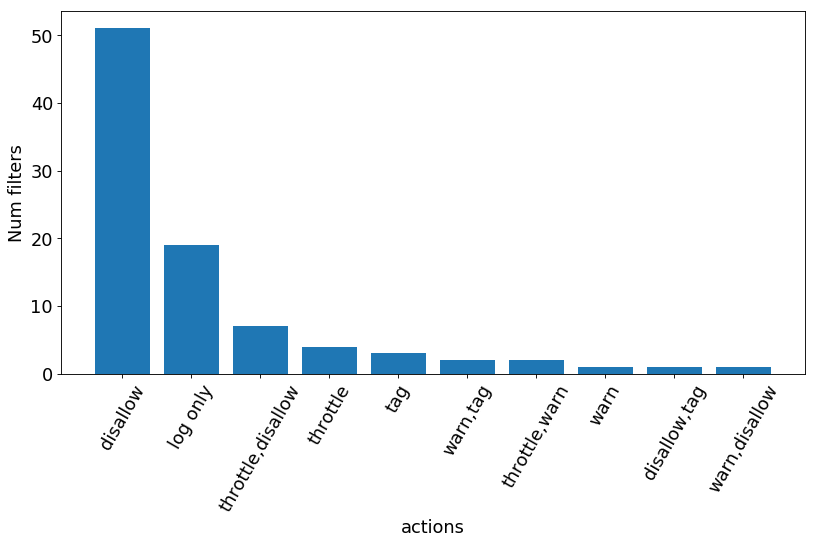
\includegraphics[width=0.9\columnwidth]{pics/active-hidden-actions-big.png}
  \caption{EN Wikipedia edit filters: Filters actions for enabled hidden filters}~\label{fig:active-hidden-actions}
\end{figure}

\subsection{What do filters target}
%: general behaviour vs edits by single users + manual tags

%TODO maybe get rid of this paragraph all together (it's partially handled by public vs private) --> merge both
As indicated in section~\ref{sec:public-hidden}, most of the public filters target disruptive behaviours in general (e.g. filter 384 disallows ``Addition of bad words or other vandalism'' by any non-confirmed user), while hidden filters are usually aimed at specific users.
There are however some public filter which target particular users or particular pages.
Arguably, (see guidelines) an edit filter may not be the ideal mechanism for this latter purpose, since every incoming edit is checked against all active filters.
In addition, time and again various filters have been introduced to track some specific sort of behaviour which was however neither malicious nor disruptive.
This contradicts/defies/fails the purpose of the mechanism and thus such filters have been (quite swiftly) disabled.
Some filters target (syn!) insults in general, and there are such which target (syn!) specifically insults aimed at particular persons (often edit filter managers).

A lot of hidden filters target specific users/problems.
\begin{comment}
  ** there are quite some filters targeting particular users: 290 (targets an IP range), 177 ('User:Television Radio'), 663 ('Techno genre warrior
', targets specific IP ranges)
  ** there are also some targetting particular pages (verify!), although this clashed with the guidelines: 264 "Specific-page vandalism" (it's hidden though, so we don't know what exactly it's doing); 401 ("Red hair" vandalism); there's smth with the main page; 715 "IP notification on RFP/C"
  ** there are also filters such as 199 (Unflagged bots) which were implemented in order to track something which was not quite malicious or abusive and were thus deemed inappropriate use of filters by the community and consequently (quite swiftly) deleted
  ** some target insults in general and some contain regexes containing very specifically insults directed towards edit filter managers (see filter 12)
\end{comment}

As figures~\ref{fig:manual-tags-all} and \ref{fig:manual-tags-active} demonstrate, the majority of filters seem to target vandalism (little surprise here).
The second biggest category comprise the ``good faith'' filters. %TODO so?
The proportion of vandalism related filters is higher when we look at all filters compared to the enabled ones.
Again, this is probably due to the presumed higher fluctuation rates of hidden filters which are always vandalism related.
It also comes to attention that the relative share of maintenance related filters is higher when we look at all filters.
The detailed distribution of manually assigned codes and their parent categories can be view on figure~\ref{fig:manual-tags}.
%TODO I don't have anything else to say here?

%TODO make these two subfigures of the same figure
\begin{figure}
\centering
  \includegraphics[width=0.9\columnwidth]{pics/donut-manual-tags-all.png}
  \caption{Manual tags parent categories distribution: all filters}~\label{fig:manual-tags-all}
\end{figure}

\begin{figure}
\centering
  \includegraphics[width=0.9\columnwidth]{pics/donut-manual-tags-active.png}
    \caption{Manual tags parent categories distribution: enabled filters (Jan 2019)}~\label{fig:manual-tags-active}
\end{figure}

\begin{landscape}
\begin{figure}
\centering
  \includegraphics[width=1\columnwidth]{pics/manual-tags-distro.png}
  \caption{Edit filters manual tag distribution}~\label{fig:manual-tags}
\end{figure}
\end{landscape}


\subsection{Who trips filters}

As of March 15, 2019 $16,489,266$ of the filter hits were caused by IP users, whereas logged in users had tripped a filter $6,984,897$ times.
A lot of the logged in users have newly created accounts (many filters look for newly created or not confirmed accounts in their pattern). %TODO what is confirmed exactly.
A user who just registered an account (or who doesn't even bother to) is rather to be expected to be inexperienced with Wikipedia, not familiar with all policies and guidelines and perhaps nor with MediaWiki syntax.

It is also quite likely (to be verified against literature!) that majority of vandalism edits come from the same type of newly/recently registered accounts.
In general, it is rather unlikely that an established Wikipedia editor should at once jeopardise the encyclopedia's purpose and start vandalising.
Although apparently there are determined trolls who ``work accounts up'' to admin and then run rampant.

%TODO mention filters discriminate towards new users: ``!(""confirmed"" in user_groups)'' is the first condition for a lot of them

\section{Filter activity}
\label{sec:filter-activity}

\subsection{Distinct filters over the years}
Thanks to quarry~\footnote{\url{https://quarry.wmflabs.org/}}, we have the numbers of all distinct filters triggered per year
from 2009 (when filters were first introduced/the MediaWiki extension was enabled) until the end of 2018: see table~\ref{tab:active-filters-count}.
This figure varies between $154$ in year 2014 and $254$ in 2018.
The explanation for this not particularly wide range of active filters lies probably in the so-called condition limit.
According to the edit filters' documentation~\cite{Wikipedia:EditFilterDocumentation}, the condition limit is a hard-coded treshold of total available conditions that can be evaluated by all active filters per incoming edit.
Currently, it is set to $1,000$.
The motivation for this heuristic is to avoid performance issues since every incoming edit is checked against all currently enabled filters which means that the more filters are active the longer the checks take.
However, the page also warns that counting conditions is not the ideal metric of filter performance, since there are simple comparisons that take significantly less time than a check against the \emph{all\_links} variable for example (which needs to query the database)~\cite{Wikipedia:EditFilterDocumentation}.
Nevertheless, the condition limit seems to still be the heuristic used for filter performance optimisation today.

\begin{table}
  \centering
  \begin{tabular}{l r }
    % \toprule
    Year & Number of distinct filters \\
    \hline
    2009 & 220 \\
    2010 & 163 \\
    2011 & 161 \\
    2012 & 170 \\
    2013 & 178 \\
    2014 & 154 \\
    2015 & 200 \\
    2016 & 204 \\
    2017 & 231 \\
    2018 & 254 \\
    % \bottomrule
  \end{tabular}
  \caption{Count of distinct filters triggered each year}~\label{tab:active-filters-count}
\end{table}

\subsection{Filter hits per month}

We can backtrack the number of filter hits over the years on figure~\ref{fig:filter-hits}.
There is a dip in the number of hits in late 2014 and quite a surge in the beginnings of 2016, after which the overall number of filter hits stayed higher.
There is also a certain periodicity to the graph, with smaller dips in the northern hemisphere's summer months (June, July, August) and smaller peaks in autumn/winter (mostly October/November).
This tendency cannot be really observed for the overall number of edits though (see figure~\ref{fig:edits-development}).
It seems that above all editors tripping filters are on vacation.

\begin{landscape}
\begin{figure}
\centering
  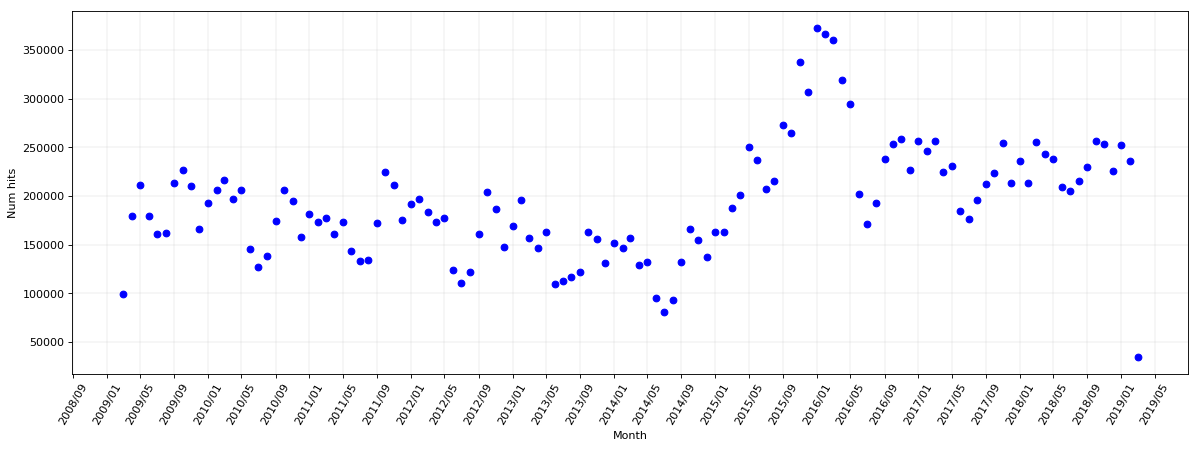
\includegraphics[width=0.9\columnwidth]{pics/filter-hits-zoomed.png}
  \caption{EN Wikipedia edit filters: Number of hits per month}~\label{fig:filter-hits}
\end{figure}
\end{landscape}

Regarding the hits surge and subsequent higher hit numbers, three possible explanations come to mind:
\begin{enumerate}
    \item the filter hits mirror the overall edits pattern from this time;
    \item there was a general rise in vandalism in this period;
    \item or there was a change in the edit filter software that allowed more filters to be activated, or a bug that caused the peak (in the form of a lot of false positives).
\end{enumerate}

I've undertaken following steps in an attempt to verify or refute each of these speculations:\\

\textbf{The filter hits mirror the overall edits pattern from this time} \\
I've compared the filter hits pattern with the overall number of edits of the time (May 2015–May 2016).
No correspondance could be determined (see figure~\ref{fig:edits-development}).
\\
\\
\textbf{There was a general rise in vandalism in this period}\\
In order to verify this assumption, it would be great to compare the filters hits patterns with revert patterns of other quality control mechanisms.
Unfortunately, computing these numbers is time-consuming and not completely trivial.
One needs a dump of English Wikipedia's edit history data for the period in question;
then one has to determine the reverts in this data set;
and then, more specifically, one needs to extract reverts done by quality control actors.
Last step is crucial, since not every revert signifies a malicious edit is being reverted.
This point is aptly illustrated by~\cite{GeiHal2017} who have demonstrated that reverts can mean productive collaborative work between different actors(syn!).

The dumps are large and it takes time and computing power to obtain them and extract reverts.
According to Geiger and Halfaker who have done this for their replication study~\cite{GeiHal2017}, the April 2017 database dump offered by the Wikimedia Foundation was 93GB compressed and it took a week to extract reverts out of it on a 16 core Xeon workstation.
They also list the challenges they faced in determining bot accounts and their reverts.

If one is to verify the current assumption (syn) properly, following steps are necessary:
\begin{enumerate}
    \item a fresh dump should be obtained
    \item reverts should be extracted from it (e.g. by using the \emph{mwreverts} python library, used also by Geiger and Halfaker
    \item reverts should be narrowed down to accounts known for doing quality-control work (for example by pre-compiling a list of anti-vandal bots); reverts (or respectively edits in general) done via Huggle and Twinkle are somewhat easy to identify since both tools leave a small code in the edit summary of their edits ("HG" for Huggle and "TW" for Twinkle)%TODO verify that's still the case
\end{enumerate}

Since time was scarce, I have run a first check of this assumption using the 2017 reverts dataset compiled by Geiger and Halfaker's for their study
\footnote{Both researchers have placed a great value on reproducibility and have published their complete datasets, as well as scripts they used for their analyses for others to use and verify: \url{https://github.com/halfak/are-the-bots-really-fighting}.}.
Figure~\ref{fig:reverts} shows the total number of reverts, as well as reverts done by bots over time computed by Geiger and Halfaker.
The filter hits pattern of 2015–2016 with the peak in filter hits and subsequent higher number of overall hits is not mirrored by the revert numbers
\footnote{Just for completenes, the spike in March 2013 is the batch action by AddBot removing interwiki links, since these were handled by Wikidata discussed in the introduction of Geiger and Halfaker's paper. It didn't have anything to do with vandalism.}
(note that the y-axis of both the revert and the filter hit plots is of the same magnitude).
As cautioned earlier, not every revert can be equated with cleaning up a disruptive edit, however, figure~\ref{fig:reverts} demonstrates that either quality control reverts constitute a relatively small portion of all reverts being done,
or that there wasn't a general surge in vandalism around this time.
(Or that only vandalism caught by filters peaked, which sounds somewhat improbable.)
\\
\\
\begin{figure}
\centering
  \includegraphics[width=0.9\columnwidth]{pics/reverts.png}
  \caption{EN Wikipedia: Revert number for the period July 2001–April 2017}~\label{fig:reverts}
\end{figure}

\textbf{There was a change in the edit filter software that allowed more filters to be activated, or a bug that caused false positives}\\
Since so far neither of the other hypothesis could be verified, this explanation sounds likely.
Another piece of data that seems to support it is the breakdown of the filter hits according to triggered filter action.
As demonstrated on figure~\ref{fig:filter-hits-actions}, there was above all a significant hits peak caused by ``log only'' filters.
As discussed in section~\ref{sec:introduce-a-filter}, it is an established praxis to introduce new filters in ``log only'' mode and only switch on additional filter actions after a monitoring period showed that the filters function as intended.
Hence, it is plausible that new filters in logging mode were introduced, which were then switched off after a significant number of false positives occured.
However, upon closer scritiny, this could not be confirmed.
The most frequently triggered filters in the period January–March 2016 are mainly the most triggered filters of all times and nearly all of them have been around for a while in 2016.
Also, no bug or a comparable incident with the software was found upon an inspection of the extension's issue tracker~\cite{phab-abusefilter-2015}, or commit messages of the commits to the software done during May 2015–May 2016~\cite{gerrit-abusefilter-source}.
Moreover, no mention of the hits surge was found in the noticeboard~\cite{Wikipedia:EditFilterNoticeboard} and edit filter talk page archives~\cite{Wikipedia:EditFilterTalkArchive2016}.
The in section~\ref{sec:filter-activity} mentioned condition limit has not changed either, as far as I can tell from the issue tracker, the commits and discussion archives, so the possible explanation that simply more filters have been at work since 2016 seems to be refuted as well.

The only somewhat interesting pattern that seems to shed some light on the matter is the breakdown of hits according to the editor's action which triggered them:
There is an obvious surge in the attempted account creations in this period (see figure~\ref{fig:filter-hits-editors-actions}).
As a matter of fact, this could also be the explanation for the peak of log only hits–the most frequently tripped filter for the period January–March 2016 is filter 527 ``T34234: log/throttle possible sleeper account creations''.
It is a throttle (only) filter, so everytime an edit matches its regex pattern, a ``log only'' entry is created in the abuse log.
%it disallows every X attempt, only logging the rest of the account creations. %I think in its current form, it does not actually disallow anything, a ``disallow'' action should be enabled for this and the filter action is only 'throttle'; so in this form, it seems to simply log account creations
And the 3rd most active filter is a ``log only'' filter as well: 650 ``Creation of a new article without any categories'' (it was neither introduced at the time, nor was there any major change in the filter pattern).
Together, filters 527 and 650 are responsible for over 60\% of the ``log only'' hits in every of the months January, February and March 2016.

Another idea that seemed worth persuing was to look into the editors who tripped filters and their corresponding edits.
For the period January-March 2016 there are some very active IP editors, the top of whom (with over $1.000$ hits) seemed to be engaging exclusively in the (probably automated) posting of spam links.
Their edits however constitute some 1-3\% of all hits from the period, so the explanation ``it was viagra spam coming from Russian IPs'' is somewhat unsatisfactory.
(Yes, it was viagra spam, and yes, a ``whois'' lookup proved them to really be Russian IPs.
And, yes, whoever was editing could've also used a VPN, so I'm not opening a Russian bot fake news conspiracy theory just yet.)
A closer/more systematic scrutiny (syn!) of the editors causing the hits may be insightful though.
Right now, all the data analysed on the matter stems from the \emph{abuse\_filter\_log} table and the checks of the content of the edits were done manually on a sample basis via the web frontend of the AbuseLog~\cite{Wikipedia:AbuseLog} where one can click on the diff of the edit for edits that triggered public filters.
No simple automated check of what the offending editors were contributing was possible since the \emph{abuse\_filter\_log} table does not store the text of the edit which triggered a filter directly, but rather contains a reference to the \emph{text} table where the wikitext of all individual page revisions is stored~\cite{Wikipedia:TextTable}.
One needs to join the hit data from \emph{abuse\_filter\_log} with the \emph{text} table to obtain the content of the edits.

Last but not least, I took a step back and contemplated the significant geo/socio-political events from the time, which triggered a lot of media (and Internet) attention and desinformation campaigns.
Following things came to mind: 2016 US elections, the Brexit referendum and the so-called ``refugee crisis'' in Europe.
There was also a severe organisational crisis in Wikimedia at the time during which a lot of staff left and eventually the executive director stepped down.

However, I couldn't draw a direct relationship between any of these political events and the edits which triggered edit filters.
An investigation into the pages on which the filters were triggered proved them (the pages) to be quite innocuous:
the page where most filter hits were logged in January 2016 (beside the login page, on which all account creations are logged) was ``Skateboard'' and the $660$ filter hits here seem like a drop in the ocean compared to the $372.907$ hits for the whole month.
And the most triggered page in March (apart from the user login page) was the user page for user 209.236.119.231 who was also the editor with second most hits and who was apparently trying to post spam links on his own user page (after posting twice to ``Skateboard'').
%Should I even mention this at all?

\begin{figure}
\centering
  \includegraphics[width=0.9\columnwidth]{pics/patterns-filterhits-actions.png}
  \caption{EN Wikipedia edit filters: Number of hits per month according to filter action}~\label{fig:filter-hits-actions}
\end{figure}

\begin{figure}
\centering
  \includegraphics[width=0.9\columnwidth]{pics/patterns-filterhits-editor-actions.png}
  \caption{EN Wikipedia edit filters: Number of hits per month according to triggering editor's action}~\label{fig:filter-hits-editors-actions}
\end{figure}

\subsection{Most active filters of all times}
\label{sec:most-active-all-times}

The ten most active filters of all times (with number of hits, public description, enabled filter actions, and the manual tag and parent category assigned during the coding described in section~\ref{sec:manual-classification}) are displayed in table~\ref{tab:most-active-actions}.
For a more detailed reference, the ten most active filters of each year are listed in the appendix. %TODO are there some historical trends we can read out of it?

Already, a couple of patterns draw attention when we look at the table:
The most active filters seem to catch a combination of possibly good faith edits which were none the less unconstructive (such as removing references, section blanking or large deletions)
and what the community has come to call ``silly vandalism''~\cite{Wikipedia:VandalismTypes} (see also code book in appendix~\ref{app:code_book}): repeating characters and inserting profanities.
Interestingly, that's not what the developers of the extension believed it was going to be good for:
``It is not, as some seem to believe, intended to block profanity in articles (that would be extraordinarily dim), nor even to revert page-blankings, '' claimed its core developer on July 9th 2008~\cite{Wikipedia:EditFilterTalkArchive1Clarification}.
Rather, among the 10 most active filters, it is filter 527 ``T34234: log/throttle possible sleeper account creations'' which seems to target what most closely resembles the intended aim of the edit filter extension, namely to take care of obvious but persistent and difficult to clean up vandalism.

\begin{comment}
%TODO compare with num hits/month for each parent cluster (vandalism, good faith, maintenance, unknown)
    Possible storyline:
    At the beginning the idea/motivation was to disallow directly gregarious vandalism.
    However, with difficulty to distinguish motivation and rising difficulty to keep desirable newcomers in the community, a more cautious behaviour was adopted, trying (as elsewhere as well) to assume good faith for ambiguous edits and to guide the editors towards a constructive contribution (e.g. via warnings).
    (So, there was a subtle transition in what the filters were applied for)
    See whether this theory is backed by the number of good faith filters (and the trends in their hit numbers)

%TODO reorder chapter and do manual tagging at the beginning; then assume a "from-the-general-picture-to-specific-occurences" approach:
    here,
    general: discuss the temporal trends in filter usage (num hits/month for each parent cluster)
    specific: and then have a look at the most active filters (of all times and if applicable per year) (also directly with what is their assigned manual tag)
\end{comment}

Another assumption that proved to be wrong/didn't quite carry into effect was that ``filters in this extension would be triggered fewer times than once every few hours''.
As a matter of fact, a quick glance at the AbuseLog~\cite{Wikipedia:AbuseLog} confirms that there are often multiple filter hits per minute.
%TODO compute means --> we can conclude from these numbers that the mechanism is quite actively used

\begin{table*}[t]
  \centering
    \begin{tabular}{p{1cm} r p{5cm} p{2cm} p{3cm}}
    % \toprule
        Filter ID & Hitcount & Publicly available description & Actions & Manual tag (parent category) \\
    \hline
        61 & 1,611,956 & new user removing references & tag & good\_faith\_refs (good\_faith) \\
        135 & 1,371,361 & repeating characters & tag, warn & silly\_vandalism (vandalism)\\
        527 & 1,241,576 & T34234: log/throttle possible sleeper account creations (hidden filter) & throttle & sockpuppetry (vandalism) \\
        384 & 1,159,239 & addition of bad words or other vandalism & disallow & profanity\_vandalism (vandalism) \\
        172 & 935,925 & section blanking & tag & good\_faith\_deletion (good\_faith) \\
        30 & 840,871 & large deletion from article by new editors & tag, warn & good\_faith\_deletion (good\_faith) \\
        633 & 808,716 & possible canned edit summary & tag & general\_vandalism (vandalism) \\
        636 & 726,764 & unexplained removal of sourced content & warn & good\_faith\_deletion (good\_faith) \\
        3 & 700,522 & new user blanking articles & tag, warn & good\_faith\_deletion (good\_faith) \\
        650 & 695,601 & creation of a new article without any categories & (log only) & general\_tracking (maintenance) \\
  \end{tabular}
  \caption{What do most active filters do?}~\label{tab:most-active-actions}
\end{table*}

\begin{comment}
    \item is it new filters that get triggered most frequently? or are there also very active old ones? -- we have the most active filters per year, where we can observe this. It's a mixture of older and newer filter IDs (they get an incremental ID, so it is somewhat obvious what's older and what's newer); is there a tendency to split and refine older filters?
\end{comment}

% Most active filters per year
%TODO compare with table and with most active filters per year: is it old or new filters that get triggered most often? (I'd say it's a mixture of both and we can now actually answer this question with the history API, it shows us when a filter was first created)


\section{Historical development}
\label{sec:5-history}

The present section explores qualitatively/highlights patterns in the creation and usage of edit filters.
Unfortunately, no extensive quantitative analysis of these patterns was possible, since for it, an access to the \emph{abuse\_filter\_history} table of the AbuseFilter plugin (compare section~\ref{sec:mediawiki-ext}) is needed.
Unlike the other tables of the extension, the \emph{abuse\_filter\_history} table is currently not replicated and no public dump is accessible via Wikimedia's cloud service Toolforge~\cite{Wikimedia:ToolforgeDatabases}.
This seems to have been the case in the past, however, due to security concerns the dumps were discontinued.
A short term solution to renew the public replicas was attempted but unfortunately haven't been successful yet.
That is why the present chapter only shows some tendencies observed via manual browsing of different filters' history via the exposed API endpoint which allows querying the \emph{abuse\_filter\_history} table for public filters~\cite{Wikipedia:AbuseFilterHistory}.
The discussions surrounding this issue and its progress can be viewed in the following ticket on Wikimedia's issue tracker:~\cite{phabricator}.
Hence, exploring historical patterns in detail remains one of the directions for future studies.

\subsection{What filters were implemented immediately after the launch + manual tags}
%TODO What were the first filters to be implemented immediately after the launch of the extension?
The extension was launched on March 17th, 2009.
Filter 1 is implemented in the late hours of that day.
Filters with IDs 1-80 (IDs are auto-incremented) were implemented the first 5 days after the extension was turned on (17-22.03.2009).
So, apparently the most urgent problems the initial edit filter managers perceived were:
page move vandalism (what Filter 1 initially targeted; it was later converted to a general test filter);
blanking articles (filter 3)
personal attacks (filter 9,11) and obscenities (12)
some concrete users/cases (hidden filters, e.g. 4,21) and sockpuppetry (16,17)

\subsection{Filter Usage/Activity}
%TODO decide how this fits into the overall narrative; write some kind of a fazit from this observations; also, decided whether this is the best representation or shouldn't they form a list rather

Following general filter operation practices were observed:
There are filters that have been switched on for a while, then deactivated and never activated again.
Some of them had only been active very briefly before they were switched off and deleted.
There are a couple of different reasons for that:
The edit filter managers decided not to implement the filter, because edit filters were deemed an inappropriate tool to deal with the issue at hand (e.g. filter 308 ``Malformed Mediation Cabal Requests'', 199 ``Unflagged Bots'', or 484 ``Shutdown of ClueBot by non-admin user'');
or decided to not implement the thing (that way): 290 ``172 Filter'' (catching edits about a Canadian politician coming from a certain IP range) was disabled, since relevant pages were protected;
or, because there were hardly any hits, so there wasn't really a problem at all (e.g. filter 304 ``Rayman vandalism'', 122 ``Changing Username malformed requests'', or 401 ``"Red hair" vandalism'').
This last group is possibly a result of edit filter managers implementing a filter ``just to see if it catches anything''.
It also occurs that filter managers implement a filter targeting the same phenomenon in parallel and without knowing of each other.
These duplicate cases are merged eventually, or alternatively all but one of them are switched off: filter 893 was switched off in favour of 891.
Sometimes, vandalism trends are only temporary and after a period of activity, the filters become stale.
This is also a reason for filters to be eventually powered off in order to save conditions from the condition limit.
Examples thereof are: 81 ``Badcharts'', 20 ``Saying "The abuse filter will block this"'', 663 ``Techno genre warrior''.
There are also filters that were switched off because they weren't doing what they were supposed to and only generated a big amount of false positives: filter 14 ``Test to detect new pages by new users''.
And there are filters testing a pattern which was eventually merged in another filter (e.g. filter 440 ``intextual.com markup'' was merged in filter 345 ``Extraneous formatting from browser extension'').

\begin{comment}
%TODO This is a duplicate of a paragraph in 4.5.1. Does it fit better here?
% this actually fits also in the patterns of new filters in chap.5; these are the filters introduced for couple of days/hours, then switched off to never be enabled again
Edit filter managers often introduce filters based on some phenomena they have observed caught by other filters, other algorithmic quality control mechanisms or general experience.
As all newly implemented filters, these are initially enabled in logging only mode until enough log entries are generated to evaluate whether the incident is severe and frequent enough to need a filter.
\end{comment}

Then, there are filters switched on for a while, deactivated for a while and activated again.
Sometimes because a pattern of vandalism is re-occuring, and sometimes–in order to fix technical issues with the filters: 61, 98 (was deactivated briefly since an editor found the "warn" action unfounded; re-enabled to tag), 148 ("20160213 - disabled - possible technical issue - see edit filter noticeboard - xaosflux")

Another group constitute enabled filters that have never been switched off since their introduction.
  164, 642 (if we ignore the 2min period it was disabled on 13.4.2018), 733 (2.11.2015-present), 29 (18.3.2009-present), 30 (18.3.2009-present), 33 (18.3.2009-present), 39 (18.3.2009-present), 50 (18.3.2009-present), 59 (19.3.2009-present), 80 (22.3.2009-present)
There are also some filters that have always been enabled with the exception of brief periods of time when the filter was deactivated (and the activated again), probably in order to update the conditions: 79, 135 (there were couple of others in Shirik's list, go back and look);
There seems to be a tendency that all actions but logging (which cannot be switched off) are took out, when edit filter managers are updating the regex of the filter.

\subsection{How do filters emerge?}
  ** an older filter is split? 79 was split out of 61, apparently; 285 is split between "380, 384, 614 and others"; 174 is split from 29
  ** several older filters are merged?
  ** or functionality of an older filter is took and extended in a newer one (479->631); (82->278); (358->633);
  ** new condition(s) are tested and then merged into existing filter : stuff from 292 was merged to 135 (https://en.wikipedia.org/wiki/Special:AbuseFilter/history/135/diff/prev/4408 , also from 366; following the comments from https://en.wikipedia.org/wiki/Special:AbuseFilter/292 it was not conceived as a test filter though, but it was rather merged in 135 post-factum to save conditions); 440 was merged into 345; apparently 912 was merged into 11 (but 11 still looks like checking for "they suck" only^^); in 460: "Merging from 461, 472, 473, 474, and 475. --Reaper 2012-08-17"
  ** an incident caught repeatedly by a filter motivates the creation of a dedicated filter (994)
  ** filter is shut down, because editors notice there are 2 (or more filters) that do nearly identical checks: 344 shut down because of 3

  ** "in addition to filter 148, let's see what we get - Cen" (https://en.wikipedia.org/wiki/Special:AbuseFilter/188) // this illustrates the point that edit filter managers do introduce stuff they feel like introducing just to see if it catches something


\section{Conclusions}

This chapter explored the edit filters on the Englisch Wikipedia in an attempt to determine what types of tasks these filters take over,
and how these tasks have evolved over time.

Different characteristics of the edit filters, as well as their activity through the years were scrutinised.
Three main types of filter tasks were identified: preventing/tracking vandalism, guiding good faith but nonetheless disruptive edits towards a more constructive contribution, and various maintenance jobs such as tracking bugs or other conspicuous behaviour.
Filters aimed at particularly malicious users or behaviours are as a general rule hidden, whereas filters targeting general patterns are viewable by anyone interested.
We've determined that hidden filters seem to fluctuate more, which makes sense given their main area of application.
Public filters often target (syn) silly vandalism or test type edits, as well as spam.
The latter, above all when implemented (syn) in an automated fashion, together with disallowing edits by very determined vandals handled by hidden filters are in accord with the initial aim with which the filters were introduced (compare section~\ref{section:4-history}).
Interestingly, the mechanism also ended up being quite active in preventing silly (e.g. inserting series of repeating characters) or profanity vandalism, which the community initially didn't think of as part of the filters' assignment (see section~\ref{sec:most-active-all-times}).
The third area in which filters are quite active are various types of blankings (mostly by new users) where the filters issue warnings pointing towards possible alternatives the editor may want to achieve or the proper procedure for deleting articles for instance.

The number of active filters stayed somewhat stable over time which is most probably to be attributed to the condition limit (see section~\ref{sec:filter-activity}).
However, this doesn't seem to be further disturbing the operation of the mechanism as a whole,
and %TODO better word
the edit filter managers use it as a performance heuristic to optimise conditions on individual filter, or routinely clean up (and disable) stale filters.

Regarding the temporal filter activity trends, it was ascertained that a sudden peak in filter activity (syn) took place in the end of 2015–beginnings of 2016, after which the overall filter hit numbers stayed higher than they used to be before this occurence.
Although there were some pointers towards what happened there:
a surge in account creation attempts and possibly a big spam wave (the latter has to be verified in a systematic fashion),
no really satisfying explanation of the phenomenon could be established.
This remains one of the possible direction for future studies.


%TODO is it really important to have this here?
In their 2012 paper Halfaker and Riedl propose a bot taxonomy according to which Wikipedia bots could be classified in one of the following task areas: content injection, monitoring, or curating; augmenting MediaWiki functionality; or protection from malicious activity~\cite{HalRied2012}.
And although there are no filters that inject or curate content, there are definitely filters whose aim is to protect the encyclopedia from malicious activity, and such that augment MediaWiki's functionality e.g. by providing warning messages (with hopefully helpful feedback) or by tagging certain behaviours to be aggregated on dashboards for later examination.

\begin{comment}
Bot taxonomy

Task area                           | Example
-----------------------------------------------------
Content
 injection                          | RamBot
 monitoring                         | SpellCheckerBot
 curating                           | Helpful Pixie Bot ("corrects ISBNs and other structural features of articles such as section capitalization")
                                    | interlanguage bots (deprecated bc of Wikidata?)
------------------------------------------------------
                                    |
Augment MediaWiki functionality     | AIV Helperbot "turns a simple page into a dynamic
priority-based discussion queue to support administrators in their work of identifying and
blocking vandal"                    | SineBot - signs and dates comments

------------------------------------------------------

Protection from malicious activity  | ClueBot_NG
                                    | XLinkBot
\end{comment}
